\documentclass{article}
\usepackage{graphicx}
\usepackage{amsmath}
\usepackage{fontsize}
\usepackage{cite}
\usepackage{color}
\usepackage{enumitem}
\usepackage{hyperref}
\usepackage{natbib}
\usepackage{tabularx}
\usepackage{natbib}
\usepackage{ragged2e}
\usepackage{sidecap}
\usepackage{geometry}
\geometry{a4paper, top=3cm, bottom=3cm, left=3.5cm, right=3.5cm}

\renewcommand*\contentsname{Indice} %Comando per cambiare il titolo del tableofcontents
\renewcommand\refname{\large Bibliografia} %Comando per cambiare il titolo delle References

\title{\Huge\textbf{La dis-informazione}}
\author{\texttt{Alessandro Meloni 0001118676 GEPID}}
\date{10/12/2023}

\begin{document}
\begin{figure}
    \centering
    \includegraphics[width=0.8\linewidth]{Immagini/Unibo arms.png}
\end{figure}
    \maketitle
\centering\tableofcontents
\newpage \section{Introduzione}
\flushleft
\begin{justify}
    Questo articolo avrà prevalentemente la finalità di provare a mettere in chiaro cosa si intenda per disinformazione e le varie sfaccettature che questo concetto può assumere.
    Faremo in modo di dare chiarezza in quanto la disinformazione ha di per sè una finalità negativa e di sviamento da ciò che è corretto, ma anche la sua forma non sempre risulta essere compresa agli occhi dei lettori.
    Innanzitutto partiremo con una piccola descrizione del concetto di disinformazione e le sue varie sfaccettature; successivamente analizzeremo una survey effettuata da parte dell'Unesco nel 2023 e pubblicata dal \href{https://www.theguardian.com/technology/2023/nov/07/85-of-people-worry-about-online-disinformation-global-survey-finds}{The Guardian}\label{:articolo} come articolo nella loro pagina internet. Questo sarà seguito da una piccola analisi del caso italiano, così da poterci fare un'idea della tendenza di percezione di questo concetto da parte della popolazione, visto che nella survey dell'UNESCO non è compresa.
    Introdurremo anche il Digital Service Act dell'UE e i suoi contenuti in merito ai Social Media.
    Seguirà successivamente una comparazione con alcuni dati relativi alla presenza oggettiva di fake news, così da capire se, in certa parte, le percezioni delle persone poi coincidono con la frequenza oggettiva del fenomeno all'interno dei vari media e l'impatto che può avere nella vita delle persone.
    In conclusione, vedremo i risultati che ha dato questa ricerca e i dati a nostra disposizione, analizzando anche il report di WEARESOCIAL del 2022 (ultimo a disposizione), così da dare dei consigli su come riconoscere informazioni da dis-informazioni, con lo scopo di creare una maggiore consapevolezza e sicurezza nell'utente/lettore medio, evitando che questo fenomeno possa davvero portare al fine per cui la notizia viene diffusa.
\end{justify}

\begin{center}
\section{Il fenomeno della disinformazione}
\end{center}

\begin{justify}
    La disinformazione è quel fenomeno che viene studiato prevalentemente negli ambiti di scienze della comunicazione, ma che può espandersi a tanti altri rami.
    L'etimologia del termine risale al 1980, appunto perché venne per la prima volta utilizzato il termine russo \textit{dezinformatzija}, che si riferisce a ‘‘un'arma’’ che venne istituita dal KGB, e che consisteva semplicemente nel creare un ufficio ad hoc finalizzato alla diffusione e gestione della disinformazione, come attività di intelligence.\citep{DisWiki}\\
    Quindi dalla creazione dell'ufficio, iniziò a diffondersi questa terminologia, andando a colpire tutti gli Stati mondiali, chi più e chi meno.
\end{justify}

\centering\subsection{Cos'è la disinformazione?}

\begin{justify}
    La disinformazione è un concetto molto ampio e bisogna subito mettere in chiaro il fatto che non si riferisca esclusivamente a intenzioni malevoli, di fatto, è giusto, come definito dalla sociologa \texttt{Claire Wardle}, suddividere questo concetto in tre ramificazioni, comprendendo:
\begin{itemize}
    \item Disinformazione: la diffusione di notizie false con lo scopo specifico di trarre in inganno e sviare singoli soggetti, organizzazioni di persone o popolazioni intere: molte volte con finalità strettamente collegate ad ambito politico, finanziario ed interessi egoistici.
    \item Misinformazione: questo termine viene preso dall'inglese ‘‘misinformation’’ e indica un'informazione che di per sè è falsa, ma senza l'effettiva finalità di nuocere altrui soggetti da parte di colui o coloro che la diffondono. Certe volte è collegata alla diffusione di pezzi di informazione di un contenuto più ampio, senza sapere che esiste questo contenuto;
    \item Malinformazione: questo termine si distacca dalla normale definizione di ‘‘notizia falsa’’, però è opportuno ricomprenderla perchè ha come contenuto una notizia vera, ma che viene diffusa senza specificare il contesto, così da arrecare danno ad uno specifico soggetto o soggetti coinvolti nella notizia. \citep{wardle2018information}
\end{itemize}
\end{justify}

\newpage\centering\subsection{Analisi dati:}

\begin{justify}    
Come già accennato nell'introduzione andremo ad analizzare precisamente una sezione della survey che è stata condotta da parte dell'UNESCO in collaborazione con IPSOS, i cui dati sono stati raccolti dal 22 Agosto al 25 Settembre 2023 e pubblicati dal The Guardian in data 7 Novembre 2023\ref{:articolo}. \citep{Unesco}
Il campione analizzato è stato formato da 500 soggetti per ogni Stato dei 16 coinvolti, per una totalità campionaria di 8000 soggetti (con un totale di popolazione pari a \textit{2.579.400.000}).
Questi 16 Stati sono stati suddivisi sulla base del loro HDI (indice di sviluppo umano), e, ogni Stato, è stato scelto in previsione delle elezioni del 2024 (infatti vediamo che non è presente l'Italia).
Come definito dall'UNESCO, la finalità è stata quella di visualizzare e analizzare, dando voce ai cittadini, quanto venga percepito l'impatto della disinformazione e degli \textit{hate speech} durante la loro vita quotidiana. D'altro canto, molto importante, è stata la decisione di fare questa survey prima delle elezioni, proprio per comprendere se in questi casi potrebbe essere sentita una maggiore diffusione di questi due fenomeni.
\end{justify}

\centering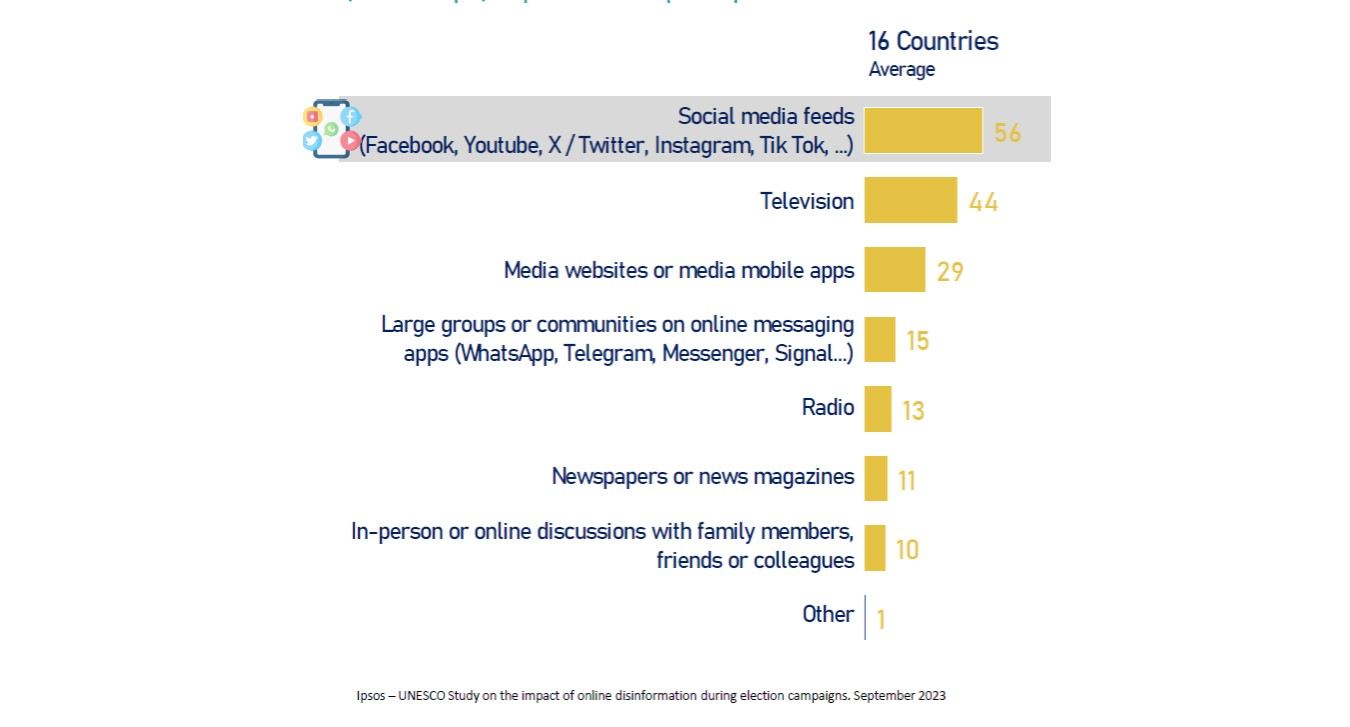
\includegraphics[width=0.6\linewidth]{Immagini/Grafico1.jpg}\\
    \begin{justify}
    Questo è il primo grafico che andremo ad analizzare dalla quale è stata posta la seguente domanda: ‘‘Qual è lo strumento che utilizzi di più per reperire news e informazioni?’’.
    Innanzitutto vediamo che gli strumenti che prevalgono sono i social network, con un distacco abbastanza sostanzioso dalla TV o altre Media inseriti all'interno dello stesso. Sicuramente questo sottolinea come, con l'avvento della digitalizzazione e dei social, le persone tendano più a informarsi con queste tecnologiche, perchè è molto più facile e veloce reperire le informazioni, visto che possono essere consultate in qualsiasi momento, al contrario della TV, perchè dovresti andare al canale specifico e aspettare che facciano rivedere il servizio.
    
\begin{center}
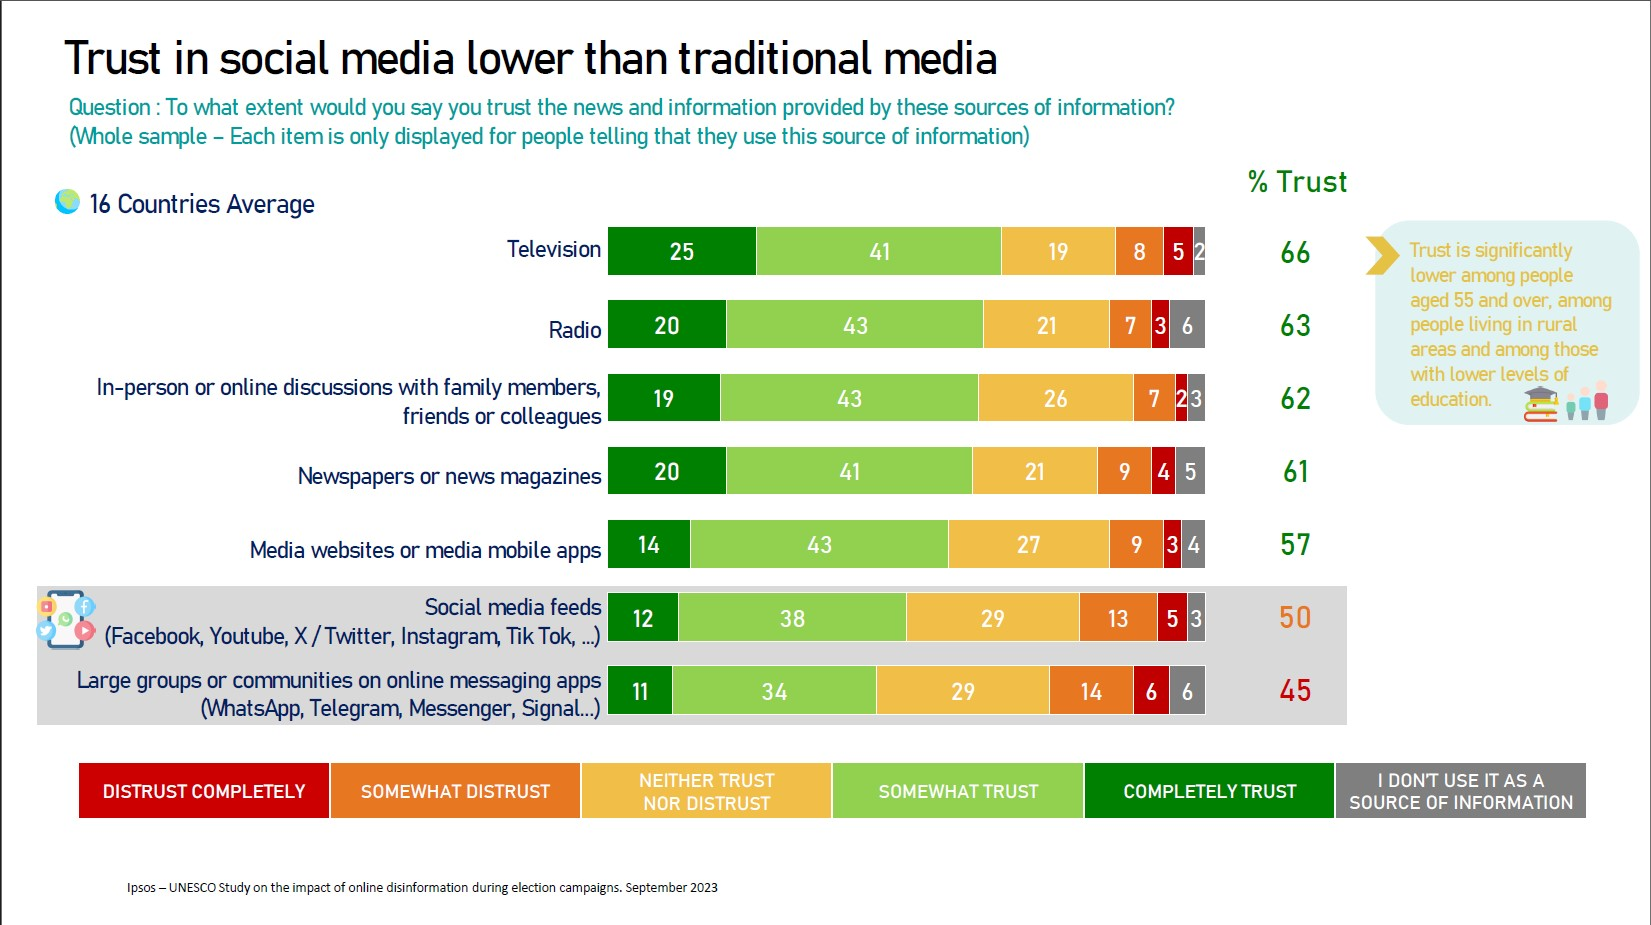
\includegraphics[width=0.6\linewidth]{Immagini/Grafico2.jpg}\\
\end{center}
    Oltre al fatto di capire come le persone si informano, bisogna comprendere anche il grado di fiducia che gli utenti danno a queste informazioni; invero, il secondo grafico rappresenta il grado di fiducia che le persone hanno rispetto agli stessi media che sono stati proposti nella prima domanda.
    Attraverso una scala nominale inserita in riferimento a questa domanda, è stato dato maggiore spazio di risposta agli intervistati (metodo che vedremo verrà confermato anche in alcuni dei prossimi grafici).
    Già da qua vediamo un controsenso, perchè gli intervistati si fidano di più dei media televisivi, radio, discussioni offline, giornali fisici e online; rispetto ai social media; mentre prima i social erano considerati come il mezzo prevalente nel reperire informazioni. A rigor di logica, quello che utilizzi di più dovrebbe coincidere anche con quello di cui ti fidi di più, invece in questo caso non accade. Potremmo intuire che i social vengano utilizzati più in maniera ricreativa e ludica, ed è per questo che si presenta questa contraddizione.
    
\begin{center}
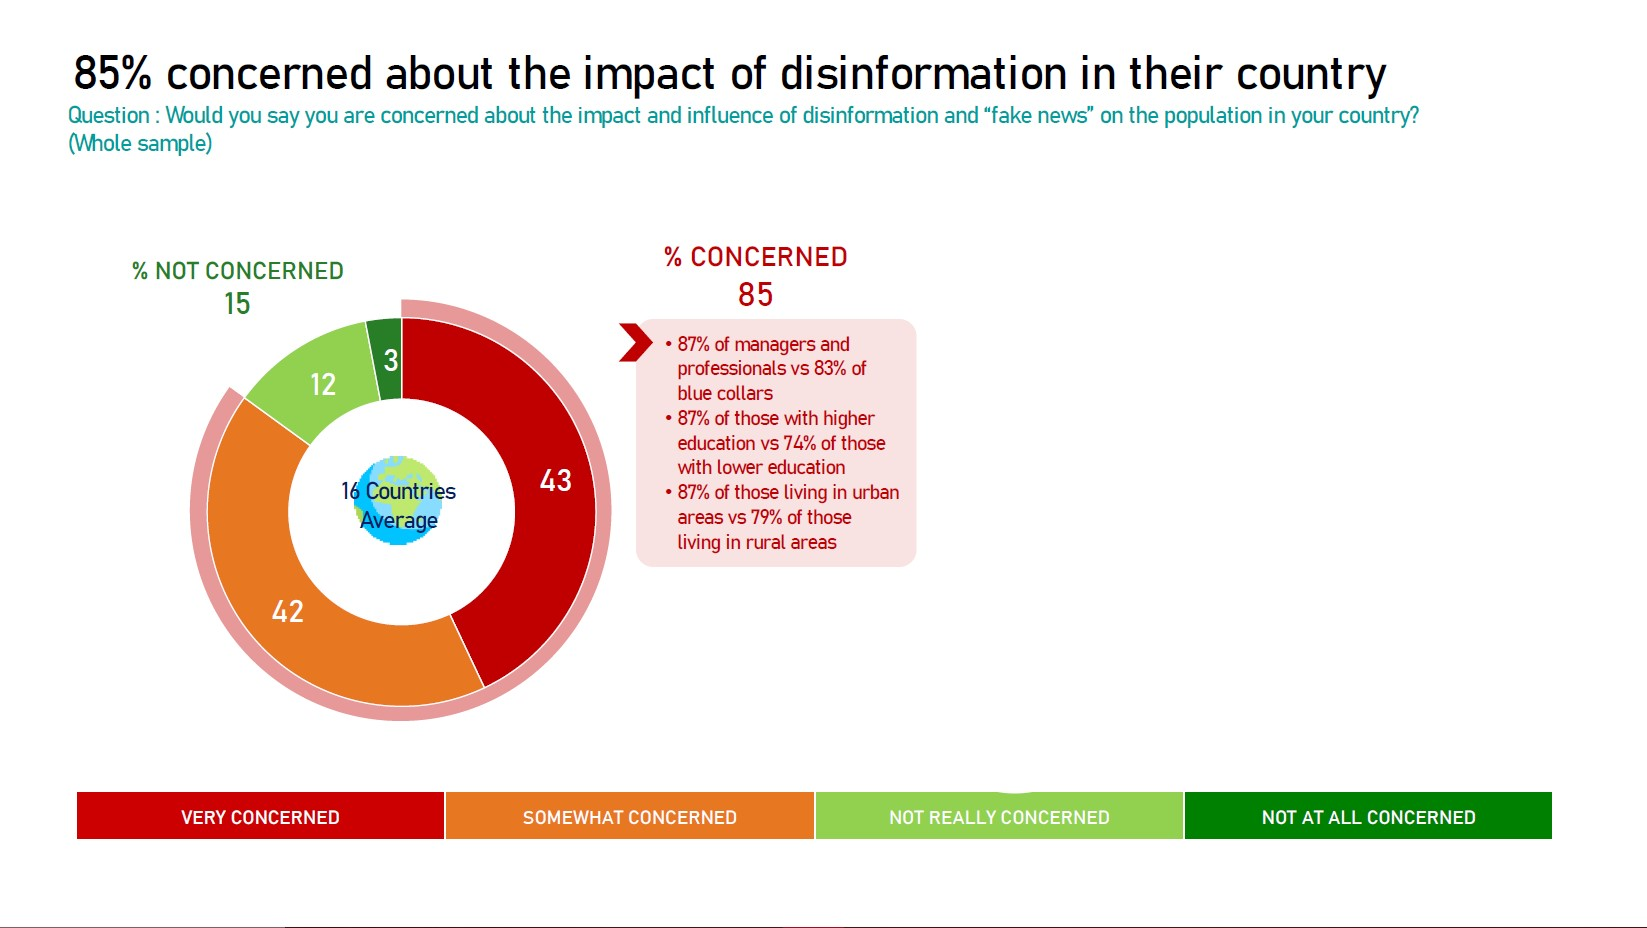
\includegraphics[width=0.6\linewidth]{Immagini/Grafico3.jpg}
\end{center}
    D'altro canto il terzo grafico continua la logica seguita, dove appunto viene chiesto quanto le persone siano preoccupate in riferimento alla disinformazione e le fake news nel proprio paese.
    Il dato che subito balza all'occhio è la stragrande prevalenza degli utenti ‘‘molto preoccupati’’ (43\%) e ‘‘abbastanza preccupati’’ (42\%). Questo dimostra che risulta esserci una forte percezione negativa del fenomeno, contando la suddivisione dei due gruppi.

\begin{center}
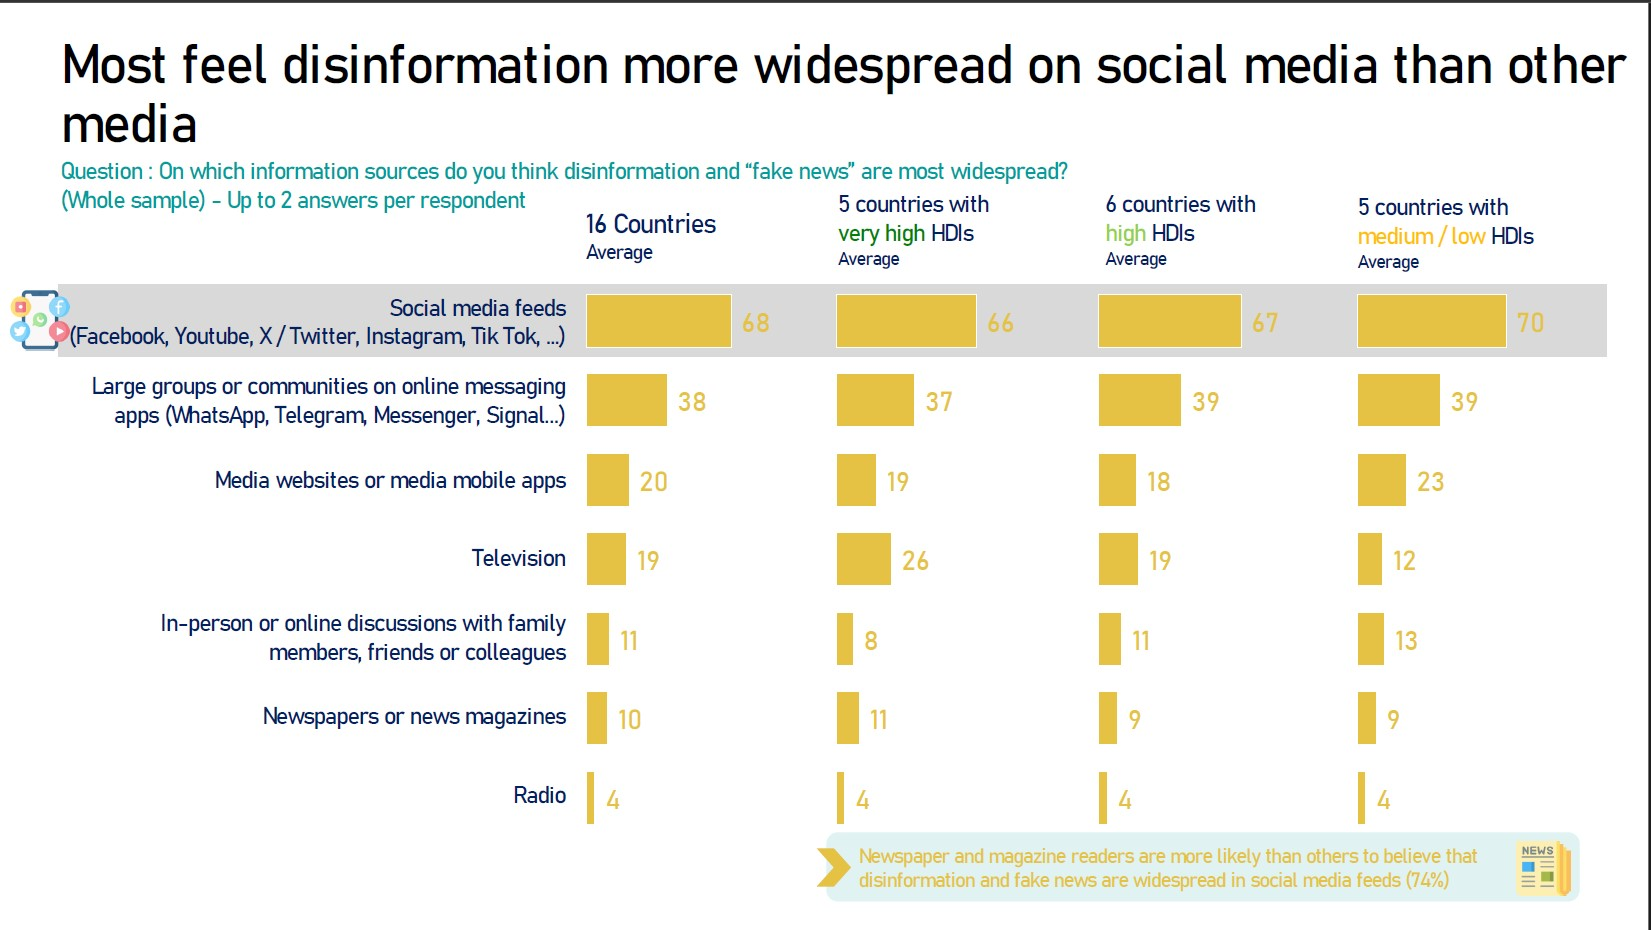
\includegraphics[width=0.6\linewidth]{Immagini/Grafico4.jpg}
\end{center}
    A questo punto bisogna comprendere dove gli utenti sentono che la disinformazione è più diffusa. Attraverso questo grafico, osserviamo che i social sono quelli che prevalgono, con una percentuale molto più alta anche solo dal secondo posto. Questo va a confermare il trend dei grafici precedenti.\\
    \\
    Come già accennato all'inizio, l'Italia non è presente all'interno di questo sondaggio, ma comunque non ci discostiamo dalla tendenza presente in questi dati.
    Di fatto, secondo il \textit{3° Rapporto Ital-Communication Censis}, circa il 83\% degli italiani utilizza il web per informarsi e il 74\% i media tradizionali: dunque, i dati seguono la falsariga di quelli intervistati dall'UNESCO.
    In più, circa il 76\% degli Italiani pensa che le fake news siano diventate difficili da rilevare, anche a causa dell'avvento di sistemi più sofisticati come le AI (lo pensa il 75\%); allo stesso modo c'è anche positività nell'utilizzo di questa tecnologia, con circa il 59\% che suppone possa garantire ulteriori strumenti per riuscire a riconoscerle.
    Infine, collegandoci a questi ultimi dati, una percentuale pari al 20\%, afferma di non avere le conoscenze per poterle distinguere.\citep{chiariello_disinformazione_2023}
\end{justify}

\centering\newpage\subsection{Digital Service Act e Social Media}
\begin{justify}
    Collegandoci a come viene percepita la disinformazione da parte dell'utente, vediamo che l'UE è intervenuta in quest'ambito con l'introduzione del \textit{Digital Service Act}: il Regolamento UE 2065/2022.\\
    Questo regolamento ha portato una rivoluzione normativa con ulteriori documenti e aggiornamenti di documenti già esistenti.
    Entrato in vigore il 25 Agosto 2023, la finalità per cui è stato istituito è proprio quella di garantire nuove istanze di trasparenza e responsabilizzazione, favorendo informazioni pluralistiche, ma al tempo stesso ‘‘non inquinate’’.
    Sulla base delle nuove regole inserite, dall'Aprile del 2023 sono sette le società poste sotto il controllo della Commissione UE: tra le più importanti Facebook, Twitter, TikTok, Instagram e Youtube.\citep{dariano_disinformazione_2023}
    Ed è qua che si presenta il dato più allarmante per l'Italia. Secondo il primo codice di auto-disciplina presentato in riferimento al primo semestre all'UE da parte delle \textit{tech companies} sotto controllo, Meta, solo in Europa, ha rimosso 140.000 contenuti considerati\textit{dannosi per la salute, con interferenza elettorale o sui censimenti}, di cui 45.000 provengono solo da Facebook Italia: diventando il paese più esposto alle social fake news in Europa (si aggiungono anche 1900 contenuti da Instagram).\\
    Seguono poi la Germania al secondo posto con 22.000 contenuti e al terzo la Spagna con 16.000.
    Allo stesso tempo, l'Italia è al secondo posto in Europa per contenuti verificati, circa 7 mln, contro i 7.4 mln della Francia che la portano al primo posto (avendo anche un miglior rapporto tra contenuti cancellati e contenuti verificati, essendosi piazzata al quinto posto per contenuti cancellati).
    Questo evidenzia l'impegno di Meta nelle verifiche con il taglio dei contributi a canali che divulgano materiale falso, passando da 20 a 26 aziende di \textit{fact checking} e dando a milioni di utenti la possibilità di disattivare alcuni contenuti personalizzati.\citep{tg24_fake_2023}\\
    X (ex Twitter) non è stato citato nei dati, proprio perché inizialmente con la nuova proprietà targata Elon Musk ha deciso di non accettare la presentazione del codice di auto-disciplina, decidendo di adattandosi dal 25 di Agosto.\\
    Pur essendo considerata dall'UE come \textit{piattaforma con il maggior rapporto di post con cattiva informazione o disinformazione}, ha introdotto una politica che vieta agli utenti di prendere di mira chiunque attui comportamenti legati all' \textit{hatespeech}.
    Molto probabilmente queste diatribe nascono perché è conveniente per le tech companies la diffusione di questi fenomeni, giacchè, oltre a creare una maggiore diffusione del contenuto, porta anche più persone a discuterne di conseguenza le aziende guadagnerebbero di più, indipendentemente dal fatto che il contenuto sia positivo o negativo.
\end{justify}

\centering
\newpage\section{Riflessione e conclusioni}
\begin{justify}
    In conclusione, con i dati alla mano osserviamo che la situazione può essere positiva o negativa, tutto ciò dipende tanto dai punti di vista che le persone sviluppano in riferimento a determinate tematiche; sulla base di ciò possiamo affermare che le percezioni delle persone possono avvolte coincidere con la realtà.
    Secondo la ricerca \textit{Digital 2023: Global Overview report} di WEARESOCIAL è emerso che tra gli utenti online dai 16 ai 64 anni sono 5.44 miliardi le persone che hanno uno smartphone, 5.16 miliardi le persone che usano internet e 4.76 miliardi hanno un account nei social media. In aggiunta le persone utilizzano con una media giornaliera di 6 ore e 37 minuti internet, 3 ore e 23 minuti la tv (comprendendo anche broadcast e streaming che sicuramente prendono gran parte delle ore di questo gruppo), 2 ore e 31 minuti i social.\citep{WEARESOCIAL}
    Sulla base di ciò le persone passano più tempo davanti a dispositivi elettronici, in internet e nei social, ragion per cui potrebbe essere più probabile che le persone possano incappare in contenuti fuorvianti e in disinformazione. Questo se pensiamo che la correlazione tra tempo trascorso e contenuti di questo tipo possa essere positiva, ma, come ci ha insegnato la ricerca di Vaccari e Valeriani \citep{vaccari_outside_2021}, non tutto si presenta sempre come ci aspettiamo, di fatto, non avendo ricerche o dati che mettano in correlazione questi due aspetti, possiamo solo fare delle supposizioni sulla base dei dati di cui disponiamo fino ad ora.
    Però rimane il problema nel riuscire a riconoscerle, sicchè i consigli che si possono dare sono:
    \begin{enumerate}
    \item Mantenere o sviluppare un pensiero critico tale per cui ogni qualvolta si legga una notizia su internet (o in generale), ci si faccia due domande e ci si informi in materia senza sentenziare o affermare che ciò che si legge sia verità assoluta.
    \item Mai basarsi unicamente sul titolo dell'articolo, può capitare che siano titoli \textit{clickbait}, dunque è sempre meglio leggere tutte le informazioni nell'articolo e poi fare un'opportuna valutazione.
    \item Infine diversificare i propri mezzi di informazione, così da non polarizzarsi su certe idee ed avere un bagaglio di conoscenze più ampio, che potrebbe sicuramente aiutare a riconoscere ciò che è vero da ciò che è falso.
    \end{enumerate}
\end{justify}

\begin{justify}
    \bibliography{Bibliografia}
    \bibliographystyle{plain}
\end{justify}

\end{document}